\graphicspath{{chapters/gradient_descent/}}


\chapter{Efficient Algorithms for the CCA Family: Unconstrained Losses with Unbiased Gradients}\label{chap:gradient_descent}
%\epigraph{It seems easier to train a bi-directional LSTM with attention than to compute the SVD of a large matrix}{Chris Ré}\cite{gemp2021}
\minitoc
% chktex-file 44
% chktex-file 3
\section*{Preface}
The content of this chapter is based on a series of papers~\citep{chapman2022generalized, chapman2023efficient} as well as a NeurIPS workshop paper~\citep{chapman2023cca}.
I am grateful to my co-authors Lennie Wells and Ana Lawry Aguila for their contributions to this work.
In particular, Lennie's mathematical expertise improved the theoretical grounding of the idea greatly and Ana's access to the UK Biobank dataset enabled the application of our methods to a real-world biomedical dataset.
In this thesis I include much of the work from these papers, but I exclude many of Lennie's extensive proofs where I can make no claim to have contributed beyond proofreading.

\section{Introduction}

Classical algorithms for linear CCA methods require computing full covariance matrices and so scale quadratically with dimension, becoming intractable for many large-scale datasets of practical interest.
There is therefore great interest in approximating solutions for CCA in stochastic or data-streaming settings \citep{arora2012stochastic}.

\section{Background: Efficient CCA}\label{sec:background-unified}

\subsection{Challenges in Solving Generalized Eigenvalue Problems}

The GEP is often represented as \( Au = \lambda Bu \), where \( A \) and \( B \) are matrices. To generalize the dimensions of these matrices, let's denote them as \( m \times m \). This dimension \( m \) can vary based on the specific method in use. For instance, in Principal Component Analysis (PCA), represented as \acrshort{pca}, \( m \) would be equal to \( p \) since \( A \) and \( B \) are \( p \times p \) matrices. In methods like Partial Least Squares (PLS) and Canonical Correlation Analysis (CCA), represented as \acrshort{pls} and \acrshort{cca} respectively, \( m \) would be \( p_1+p_2 \), as \( A \) and \( B \) in these cases are \( (p_1+p_2) \times (p_1+p_2) \).

% Table summarizing the definitions of A and B for various methods
\begin{table}[h]
    \centering
    \begin{tabular}{|c|c|c|c|c|}
        \hline
        Method         & \( A \)           & \( B \)   & \( u \)        & Dimensions       \\
        \hline
        \acrshort{pca} & \( \Sigma_{11} \) & \( I \)   & \( u\sps{1} \) & \( p \times p \) \\
        \hline
        LDA            & \( S_B \)         & \( S_W \) & \( u\sps{1} \) & \( p \times p \) \\
        \hline
        \acrshort{cca} & \( \begin{pmatrix}
                                \Sigma_{11} & \Sigma_{12} \\ \Sigma_{21} & \Sigma_{22}
        \end{pmatrix} \) & \( \begin{pmatrix}
                                  \Sigma_{11} & 0 \\ 0 & \Sigma_{22}
        \end{pmatrix} \) & \( \begin{pmatrix}
                                  u\sps{1} \\ u\sps{2}
        \end{pmatrix} \) & \( (p_1+p_2) \times (p_1+p_2) \) \\
        \hline
        \acrshort{pls} & \( \begin{pmatrix}
                                0 & \Sigma_{12} \\ \Sigma_{21} & 0
        \end{pmatrix} \) & \( I \) & \( \begin{pmatrix}
                                            u\sps{1} \\ u\sps{2}
        \end{pmatrix} \) & \( (p_1+p_2) \times (p_1+p_2) \) \\
        \hline
    \end{tabular}
    \caption{Definitions and dimensions of \( A \)and \( B \) for different subspace learning methods.}
    \label{tab:subspace}
\end{table}

To solve the GEP, one common technique is to transform it into a standard eigenvalue problem \( B^{-\frac{1}{2}} A B^{-\frac{1}{2}} y = \lambda y \), followed by eigendecomposition.
However, this approach has computational complexity \( O((p_1+p_2)^3) \) and may suffer from numerical instability.

\subsection{\acrshort{pca}-CCA}

One way to reduce the complexity of solving GEPs is to use the \acrshort{pca}-CCA method, which first applies \acrshort{pca} to the data and then solves the GEP in the reduced space.
An important advantage of using \acrshort{pca}-CCA is computational efficiency, especially for high-dimensional data.
The overall complexity of \acrshort{pca}-CCA involves two main steps.
First, applying PCA has a complexity of \( O(p_1^3+ p_2^3) \), dominated by the larger of the two matrices.
Second, solving the generalized eigenvalue problem in the reduced space with \( K \) components in each view leads to a complexity of \( O((2K)^3) \).
Thus, the overall complexity of \acrshort{pca}-CCA is \( O(p_1^3+ p_2^3) + (2K)^3) \), which is significantly lower than the complexity of solving the GEP directly.
Since CCA, ridge CCA, and PLS can all be solved in the principal component space, \acrshort{pca}-CCA can be used to compute solutions efficiently \textit{even if we keep all the principal components}.
Most obviously, this is the case when the number of samples \( n \) is smaller than either of the number of features \( p_1 \) or \( p_2 \), i.e. \( n < p_1 \) or \( n < p_2 \).
In this case the maximum number of principal components is \( K=n \), and the complexity of PCA is \( O(n^3+ n^3) \) so that the overall complexity of \acrshort{pca}-CCA is thus \( O(2n^3+(2n^3)^3) \) = \( O(10n^3) \).
For fat data where \( p_1 \) and \( p_2 \) are larger than \( n \), we can reasonably expect $10n^3<p_1^3+ p_2^3$ and thus \acrshort{pca}-CCA is still more efficient than solving the original GEP.

We illustrate this in a simple simulation study in Figure \ref{fig:pca-cca-complexity}\footnote{This simulation was used to justify our pull request to \texttt{scikit-learn}\citep{pedregosa2011scikit} implementing a PCA-PLS and PCA-CCA backend}.

\begin{figure}
    \centering
    \includegraphics[width=0.7\textwidth]{figures/benchmarks/bench_ridgecca_pls.pdf}
    \caption{Comparison of the complexity of PCA-CCA and CCA for varying numbers of samples and features.}
    \label{fig:pca-cca-complexity}
\end{figure}

This approach has been employed to great effect in neuroimaging but suprisingly is not used even in the scikit-learn implementation of \acrshort{cca} \citep{pedregosa2011scikit}.
Nonetheless, for the large sample sizes (desirable for machine learning frameworks as well as statistical power), the complexity of even \acrshort{pca}-CCA can render the problems nearly intractable.

\subsection{Kernel CCA}

Kernel \acrshort{cca} (\acrshort{kcca}) also offers computational efficiency for high-dimensional data (\(p_i>n\)) as its complexity scales with the number of samples \(n\), not the number of features \(p_i\)\citep{akaho2006kernel}.
It casts the CCA optimisation as a dual problem:

\begin{align}
    & \alpha_{\text{opt}}=\underset{\alpha}{\mathrm{argmax}}\{ \alpha\sps{1}K\spsT{1}K\sps{2}\alpha\sps{2}  \} \\
    & \text{subject to:} \notag                                                                                            \\
    & \alpha\sps{1}K\spsT{1}K\sps{1}\alpha\sps{1}=1 \notag                                                                  \\
    & \alpha\sps{2}K\spsT{2}K\sps{2}\alpha\sps{2}=1 \notag
\end{align}

Where \(\alpha\sps{i}=\) are dual variables, \(K\sps{i}\) are kernel matrices, and \(K\spsT{i}\) are their transposes.
The kernel matrices are defined as \(K\sps{i}=\phi(X\sps{i})\phi(X\sps{i})^T\), where \(\phi(\cdot)\) is a nonlinear mapping function.
The kernel trick is used to avoid the explicit computation of the nonlinear mapping function \(\phi(\cdot)\).
The complexity of \acrshort{kcca} is \(O(n^3)\), which can be much lower than the complexity of solving the original GEP directly when \(p_i>n\).
However, a significant drawback of KCCA is the need for access to all training data at test time, which raises concerns about efficiency and scalability.
Furthermore, when the number of samples is large, the kernel matrix can itself be too large to fit in memory.

\subsection{Stochastic PLS and CCA}
Recently, a number of algorithms have been proposed to approximate GEPs including PCA and PLS \citep{arora2012stochastic}, and CCA specifically \citep{bhatia2018gen}, in the `stochastic' or `data-streaming' setting; these can have big computational savings.
Typically, the computational complexity of classical GEP algorithms is $\mathcal{O}\left((n + k)p^2\right)$; by exploiting parallelism (both between eigenvectors and between samples in a mini-batch), we can reduce this down to $\mathcal{O}\left(d k \right)$ \citep{arora2016stochastic}.
Stochastic algorithms also introduce a form of implicit regularisation \citep{smith2021origin} which can be very helpful in these high-dimensional settings.
To the best of our knowledge, the state-of-the-art in Stochastic PLS and CCA are the subspace Generalized Hebbian Algorithm (SGHA) \citep{chen2019constrained} and $\gamma$-EigenGame \citep{gemp20,gemp2021}.
\paragraph{SGHA} uses a Lagrange multiplier heuristic along with saddle-point analysis, albeit with limited convergence guarantees.
Specifically, they form the constrained optimization problem for the top-k subspace as

\begin{align}
    \min_{U} -\Tr U^T A U \quad \text{subject to} \quad U^T B U = I
\end{align}

Transforming this into an unconstrained problem using Lagrange multipliers:

\begin{align}
    \min_{U} -\Tr\left(U^T A U \right) + \lambda \left(U^T B U - I\right)
\end{align}

Finally, they combine the primal and dual updates into a single update rule:

\begin{align}
    U_{t+1} = \left(1 - \eta_t\right) U_t + \eta_t \left(A U_t + \lambda_t B U_t\right)
\end{align}

This algorithm is very simple to implement but because it is based on a heuristic primal-dual update rule rather than gradient descent, it is hard to use with more sophisticated optimizers such as Adam \citep{kingma2014adam}.

\paragraph{$\gamma$-EigenGame} is a stochastic algorithm for CCA which is based on the $\gamma$-Eigengame for PCA \citep{gemp20}.
The EigenGame series of algorithms are based on the idea of eigenvectors competing to explain the data.
They each maximize a utility function with reward and penalty terms:

\begin{align}
    \max_{u_i} \overbrace{\frac{u_i^TAu_i}{u_i^TBu_i}}^{rewards} - \overbrace{\sum_{j < i} \frac{(u_j^TAu_j)(u_i^TBu_j)^2}{(u_j^TBu_j)^2(u_i^TBu_i)}}^{penalties}
\end{align}

Where player $i$ only needs to maintain orthogonalization with respect to players $j < i$.
By a few heuristic arguments, this can be moulded to an update rule in the full batch case:

\begin{align}
    u_i \leftarrow (u_i^T B u_i)A u_i - (u_i^T A u_i)B u_i - \sum_{j < i} (u_i^T A y_j)[(u_i^T B u_i)B y_j - (u_i^T B y_j)B u_i]
\end{align}

Where $y_i = \frac{u_i}{\sqrt{u_i^TBu_i}}$. Finally, the stochastic version of this algorithm is obtained by replacing $B y_j$ with a rolling average of $B u_j$, necessitating an additional hyperparameter $\gamma$ which must be tuned. As with SGHA, this algorithm is also hard to combine with more sophisticated optimizers.

\section{Methods: Novel Objectives and Algorithms}\label{sec:contributions}

In this section, we introduce a novel class of objectives for GEPs, which we call the Eckhart--Young (EY) objectives.
They can be applied to any GEP, including CCA, PLS, and PCA but we will focus on CCA.

\subsection{Unconstrained objective for GEPs}\label{sec:gep-ey-formulation}
First, we present proposition \ref{prop:EY-charac}, a formulation of the top-$K$ subspace of GEP problems, which follows by applying the Eckhart--Young--Minsky inequality \citep{stewart_matrix_1990} to the eigen-decomposition of $B^\mhalf A B^\mhalf$. However, making this rigorous requires some technical care which we defer to the proof in supplement \ref{app:proofs}.

\begin{restatable}[Eckhart--Young inspired objective for GEPs]{proposition}{EYcharac}
    \label{prop:EY-charac}
    The top-$K$ subspace of the GEP $(A,B)$ can be characterized by minimizing the following objective over $U \in \R^{D \times K}$:
    \begin{align}\label{eq:EY-charac}
    \LEYGEP(U) \defeq \tr \left( - 2\,U^T A U + \left(U^T B U\right) \left(U^T B U\right) \right)
    \end{align}
    Moreover, the minimum value is precisely $- \sum_{k=1}^K \lambda_k^2$, where $(\lambda_k)$ are the generalized eigenvalues.
\end{restatable}

This objective also has appealing geometrical properties.
It is closely related to a wide class of unconstrained objectives for PCA and matrix completion which have no spurious local optima \citep{ge_no_2017}, i.e. all local optima are in fact global optima.
This implies that certain local search algorithms, such as stochastic gradient descent, should indeed converge to a global optimum.

\begin{restatable}{proposition}{NoSpuriousLocalMinima}[No spurious local minima]\label{prop:no-spurious}
The objective $\LEYGEP$ has no spurious local minima.
That is, any matrix $\bar{U}$ that is a local minimum of $\LEYGEP$ must in fact be a global minimum.
\end{restatable}

It is also possible to make this argument quantitative by proving a version of the strict saddle property from \cite{ge_no_2017,ge2015escaping}; we state an informal version here and give full details in \cref{supp:tractable-optimization}.

\begin{corollary}[Informal: Polynomial-time Optimization]
    Under certain conditions on the eigenvalues and generalized eigenvalues of $(A,B)$, one can make quantitative the claim that:
    any $U_K \in \R^{D \times K}$ is either close to a global optimum, has a large gradient $\nabla \LEYGEP$, or has Hessian $\nabla^2 \LEYGEP$ with a large negative eigenvalue.

    Therefore, for appropriate step-size sequences, certain local search algorithms, such as sufficiently noisy SGD, will converge in polynomial time with high probability.
\end{corollary}

\subsection{Corresponding Objectives for the CCA family}
For the case of linear CCA we have $U^T A U = \sum_{i \neq j} \Cov(Z\sps{i}, Z\sps{j}), U^T B U = \sum_{i} \Var(Z\sps{i})$.
To help us extend this to the general case of nonlinear transformations, \cref{eq:general-form-of-representations}, we define the analogous matrices of total between-view covariance and total within-view variance
\begin{align}\label{eq:def-C-V-matrices}
\vphantom{\bigl(\bigr)} % increase vertical space
C(\theta) = \sum_{i \neq j} \Cov(Z\sps{i}, Z\sps{j}), \quad
V(\theta) = \sum_{i} \Var(Z\sps{i})
\end{align}
In the case of linear transformations:

\begin{equation}\label{eq:cca-linear-function-def}
Z\sps{i}_k = \langle u_k\sps{i} , X\sps{i} \rangle.
\end{equation}

it makes sense to add a ridge penalty so we can define
\begin{align}\label{eq:v-alpha-ridge-definition}
V_\alpha(\theta) = \sum_i \alpha_i {U\spsT{i}} U\sps{i} +  (1 - \alpha_i) \Var(Z\sps{i})
\end{align}
This immediately leads to following unconstrained objective for the CCA-family of problems.
\begin{definition}[Family of EY Objectives]
    Learn representations $Z\sps{i} = f\sps{i}( X\sps{i}; \theta\sps{i})$ minimizing
    \begin{align}\label{eq:EY-loss-def-C-V}
    \LEY(\theta) = - 2 \tr C(\theta) + \norm{V_\alpha(\theta)}_F^2
    \end{align}
\end{definition}

\paragraph{Unbiased estimates}
since empirical covariance matrices are unbiased, we can construct unbiased estimates to $C, V$ from a batch of transformed variables $\Z$.
\begin{align}\label{eq:def-C-V-matrices-empirical}
\hat{C}(\theta)[\Z] = \sum_{i \neq j} \empCov(\Z\sps{i}, \Z\sps{j}), \quad
\hat{V}(\theta)[\Z] = \sum_{i} \empVar(\Z\sps{i})
\end{align}
In the linear case we can construct $\hat{V}_\alpha(\theta)[\Z]$ analogously by plugging sample covariances into \cref{eq:v-alpha-ridge-definition}.
Then if $\Z, \Z'$ are two independent batches of transformed variables, the batch loss
\begin{align}\label{eq:empirical-EY-loss-estimate-def}
\empLEY[\Z, \Z'] \defeq - 2 \tr \hat{C}[\Z] + \langle \hat{V}_\alpha[\Z], \hat{V}_\alpha[\Z'] \rangle_F
\end{align}
gives an unbiased estimate of $\LEY(\theta)$.
This loss is a differentiable function of $\Z, \Z'$ and so also of $\theta$.

\paragraph{Simple algorithms:}
We first define a very general algorithm using these estimates in Algorithm \ref{alg:general}.
In the next section we apply this algorithm to multi-view stochastic CCA and PLS.

\begin{algorithm}
    \caption{GEP-EY: General algorithm for learning correlated representations}
    \label{alg:general}
    \begin{algorithmic}
        \STATE {\bfseries Input:} data stream of mini-batches $(\X(b))_{b=1}^\infty$ where each consists of $M$ samples from the original dataset. Learning rate $(\eta_t)_t$. Number of time steps $T$. Class of functions $f(\cdot; \theta)$ whose outputs are differentiable with respect to $\theta$.
        \STATE {\bfseries Initialize:} $\hat{\theta}$ with suitably random entries
        \FOR{$t=1$ {\bfseries to} $T$}
        \STATE Obtain two independent mini-batches \( \X(b), \X(b') \) by sampling \( b, b' \) independently
        \STATE Compute batches of transformed variables $\Z(b) = f(\X(b); \theta), \Z(b') = f(\X(b'); \theta)$
        \STATE Estimate loss $\empLEY(\theta)$ using \cref{eq:empirical-EY-loss-estimate-def}
        \STATE Obtain gradients by back-propagation and step with your favourite optimizer.
        \ENDFOR
    \end{algorithmic}
\end{algorithm}

\subsection{Applications to (multi-view) stochastic CCA and PLS}
\begin{lemma}[Objective recovers GEP formulation of linear (multi-view) CCA]
    When $f\sps{i}$ are linear, as in \ref{eq:cca-linear-function-def}, the population loss from \cref{eq:EY-loss-def-C-V} recovers MCCA.
\end{lemma}
\begin{proof}
    By construction, for linear MCCA we have $C = U^T A U,\, V_\alpha=U^T B_\alpha U$, where $(A, B_\alpha)$ define the GEP for MCCA introduced in \cref{eq:gep-most-general-formulation}.
    So $\LEY(U) = \LEYGEP(U)$ and by \cref{prop:EY-charac} the optimal set of weights define a top-$K$ subspace of the GEP, and so is a MCCA solution.
\end{proof}

Moreover, by following through the chain of back-propagation, we obtain gradient estimates in $\mathcal{O}(MKD)$ time.
Indeed, we can obtain gradients for the transformed variables in $\mathcal{O}(M K^2)$ time so the dominant cost is then updating $U$; we flesh this out with full details in \cref{supp:fast-updates}.

\section{Experiments}

\subsection{Stochastic CCA}
In this study, we aim to demonstrate that our proposed CCA-EY method not only matches but potentially surpasses the performance of established baselines $\gamma$-EigenGame and SGHA in terms of convergence speed and robustness to hyperparameter settings. Our experimental setup largely follows the framework established by \citet{meng2021online, gemp2022generalized}. A key distinction in our approach, however, is the decision to not perform PCA on the data prior to applying CCA methods. This choice retains the full complexity of the datasets, providing a more rigorous evaluation of each algorithm's ability to handle high-dimensional data efficiently and accurately.

One of the central goals of this comparison is to illustrate that CCA-EY can achieve faster convergence with less hyperparameter tuning, an essential attribute for practical applications. To facilitate a fair and direct comparison with the baseline methods, we employ Stochastic Gradient Descent (SGD) as the optimization technique for all algorithms. It is worth noting that while SGD provides a baseline for performance assessment, the potential of our CCA-EY method could be further unleashed by utilizing more advanced optimization techniques such as momentum-based optimizers like Adam or Nesterov acceleration. These advanced methods are known for their ability to accelerate convergence and navigate the optimization landscape more effectively, suggesting that our method might yield even better performance under such enhanced optimization schemes.

We train models to optimize CCA on the MediaMill and Split-CIFAR-10 datasets for a single epoch, using mini-batch sizes ranging from 5 to 100. These sizes were selected to test the scalability and efficiency of our method under varied computational loads. The Proportion of Correlation Captured (PCC) metric, defined as \( \text{PCC} = (\sum_{i=k}^K \rho_k)/ ({\sum_{k=1}^K \rho_k^*}) \), serves as our evaluation criterion. Here, $\rho_k$ represents the correlations of the estimated representations $Z\sps{i}=X^{(i)}\hat{U}^{(i)}$ with one another on the test set, while $\rho_k^*$ denotes the canonical correlations computed from the full batch covariance matrices. Despite $\rho_k^*$ not being the `true` correlations, their computation from a large sample size renders them a reliable benchmark. PCC is an efficient metric for tracking algorithmic performance over time, minimizing computational overhead\citep{meng2021online, gemp2022generalized, ma2015finding, ge2016efficient}.

\paragraph{Data}
The MediaMill dataset \citep{gemert2008visual} comprises paired features of videos and corresponding commentary, with the objective of learning joint representations that capture their correlation. This representation could potentially enable prediction of commentary from video, or vice versa. The dataset includes 25,800 test images, with 120 and 101 features respectively.

The Split-CIFAR dataset \citep{meng2021online} consists of 50,000 training and 10,000 test RGB images, each split in half with 32x16x3 features. The aim is to learn joint representations of the two halves that reveal correlations, expected to be high within the same class and low across different classes. These datasets are chosen for their diverse nature and complexity, providing a comprehensive test bed for our method.

\paragraph{Parameters} For each method, we searched over the hyperparameter grid in table \ref{tab:hyperparameters} using \citet{wandb}.

\begin{table}[h!]
    \centering
    \begin{tabular}{|l|l|}
        \hline Parameter             & Values              \\
        \hline minibatch size        & 5,20,50,100         \\
        \hline components            & 5                   \\
        \hline epochs                & 1                   \\
        \hline seed                  & 1, 2, 3, 4, 5       \\
        \hline lr                    & 0.01, 0.001, 0.0001 \\
        \hline $\gamma$\footnotemark & 0.01,0.1,1,10       \\
        \hline
    \end{tabular}
    \footnotetext{gamma is only used for $\gamma$-EigenGame}\label{tab:hyperparameters}
\end{table}

\paragraph{Observations}
For the MediaMill dataset, Figure \ref{fig:corr_mediamill} compares the algorithms' performance across various mini-batch sizes, showing CCA-EY's consistent outperformance. Figure \ref{fig:learningcurve_mediamill} further examines the learning curves for batch sizes 5 and 100, illustrating CCA-EY's superior performance over time.

\begin{figure}
    \centering
    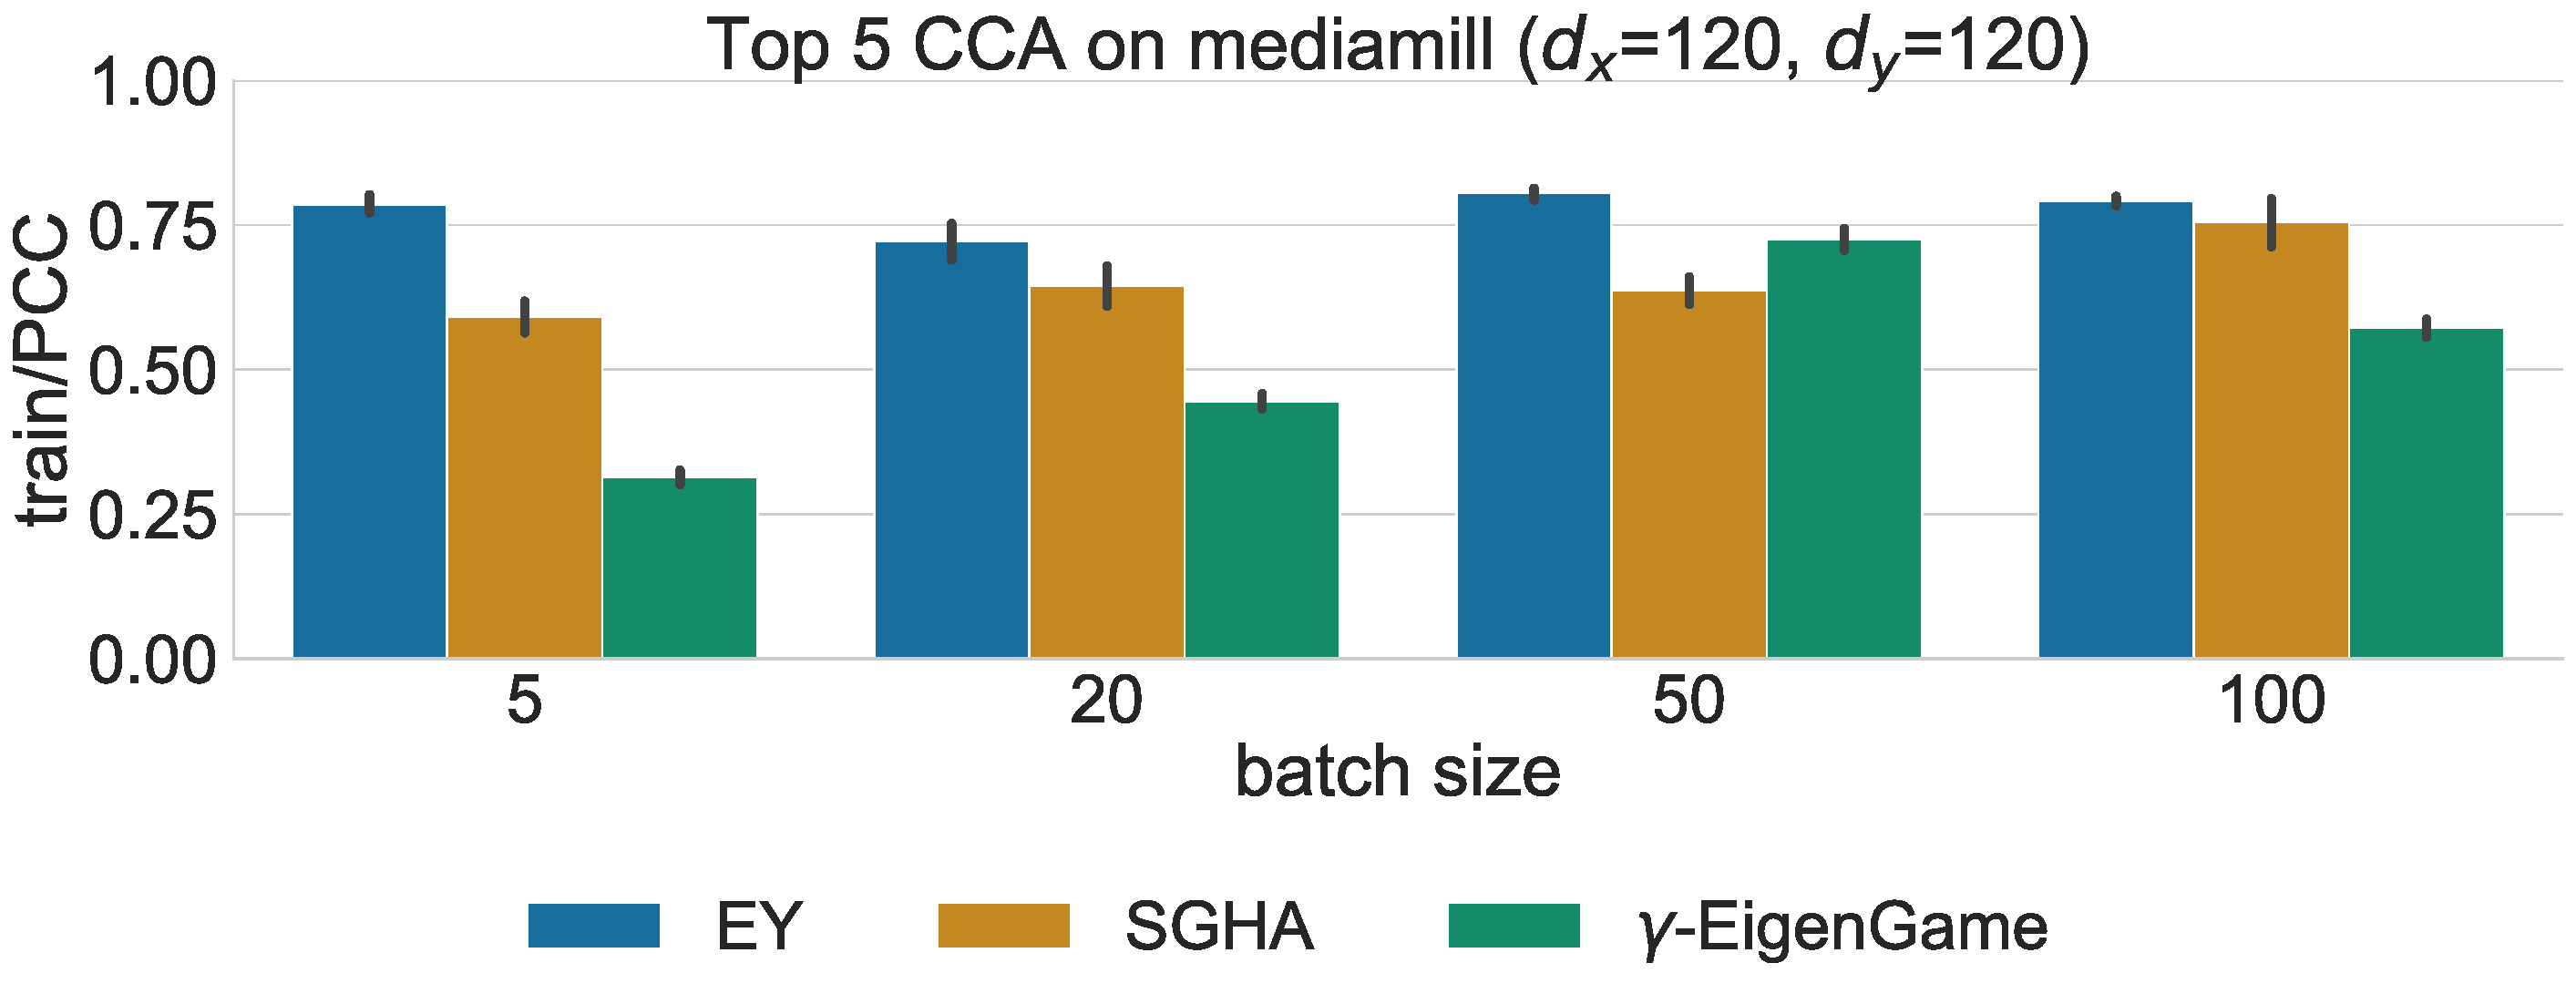
\includegraphics[width=0.6\textwidth]{figures/CCA/mediamill_models_different_batch_sizes}
    \caption{Stochastic CCA on MediaMill using PCC: Performance across varying mini-batch sizes. Shaded regions signify \(\pm\) one standard deviation around the mean of 5 runs.}
    \label{fig:corr_mediamill}
\end{figure}

\begin{figure}
    \centering
    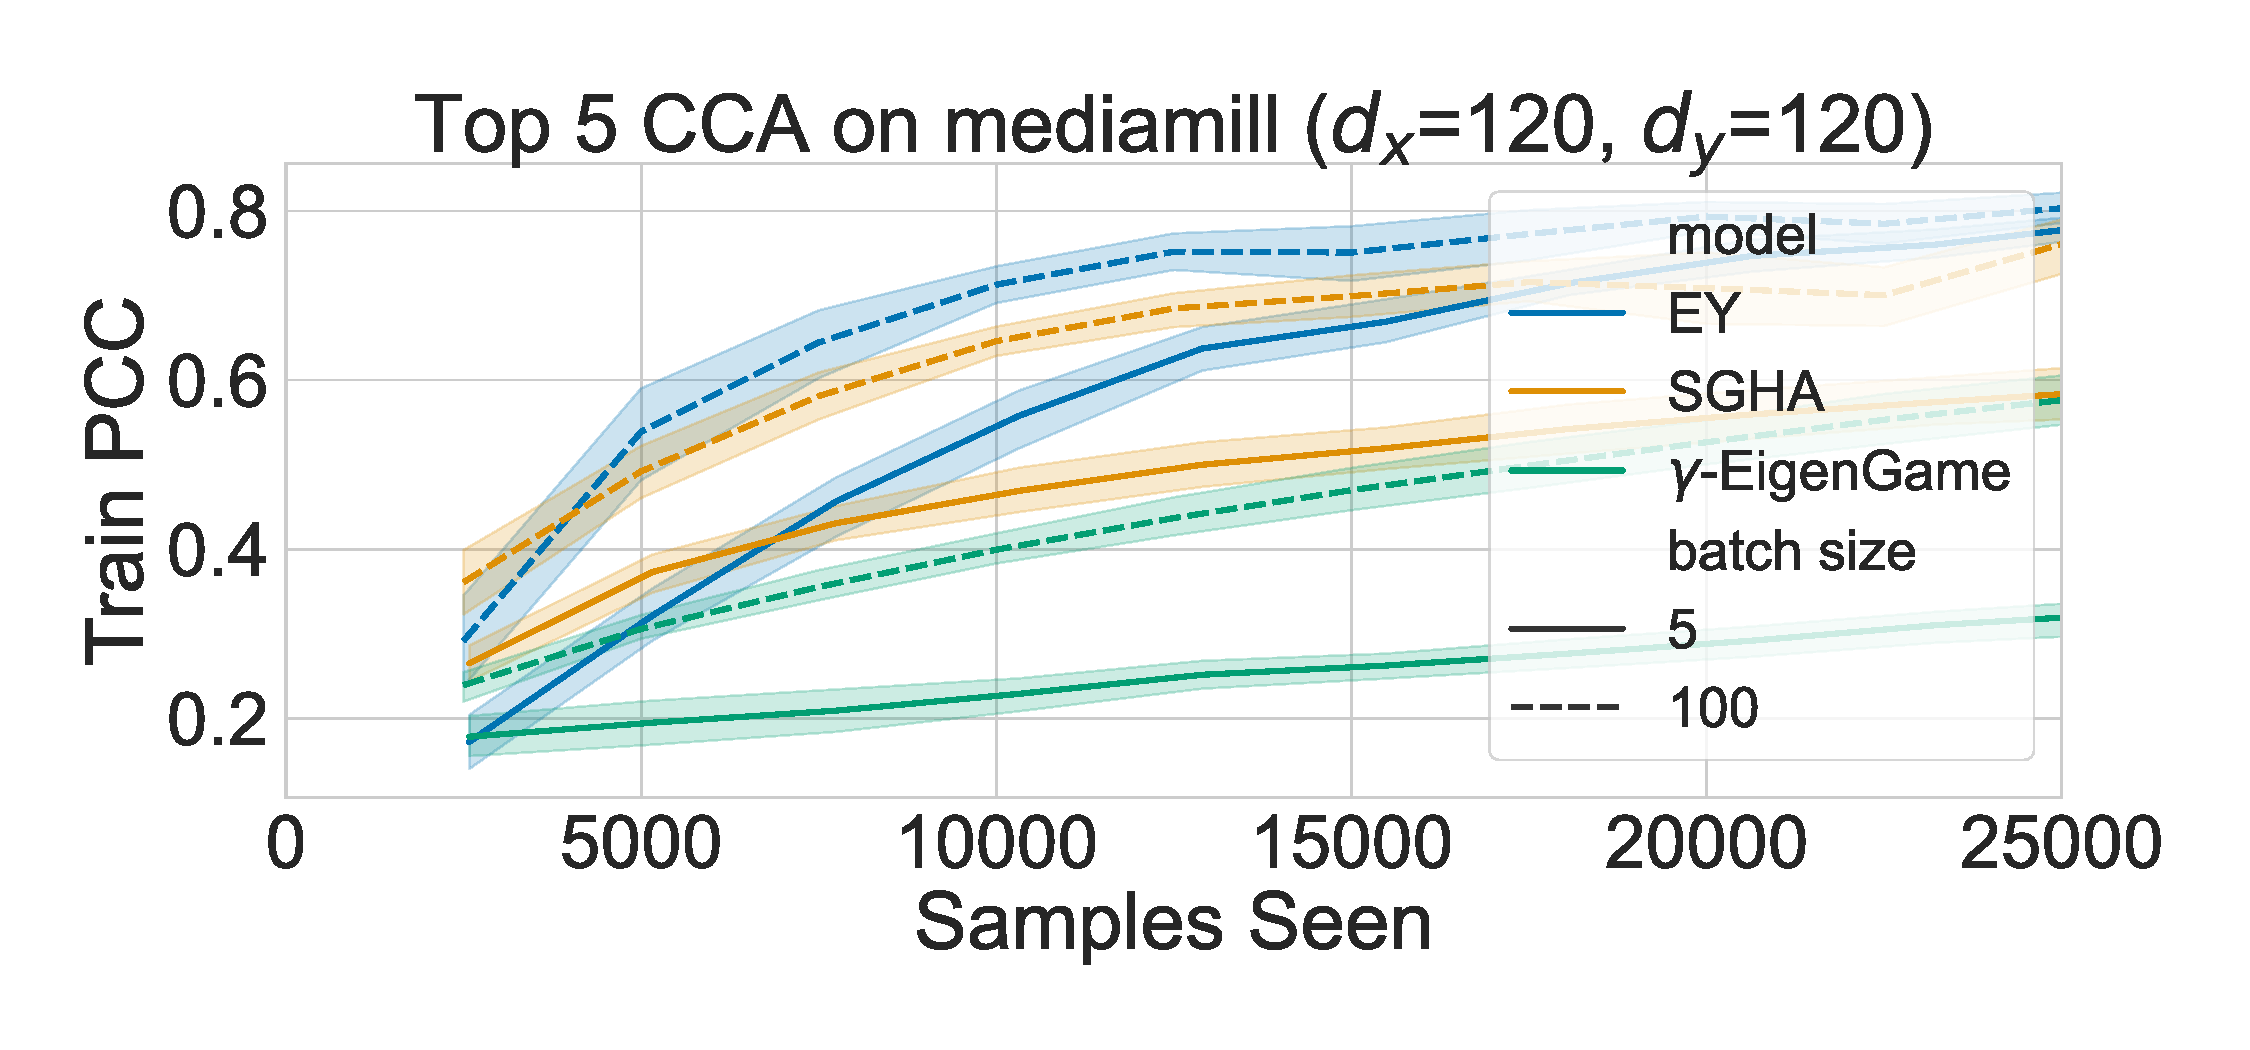
\includegraphics[width=0.6\textwidth]{figures/CCA/mediamill_allbatchsizes_pcc}
    \caption{Stochastic CCA on MediaMill: Training progress over a single epoch for mini-batch sizes 5, 100.}
    \label{fig:learningcurve_mediamill}
\end{figure}

For the CIFAR dataset, Figure \ref{fig:corr_cifar} shows the performance comparison across batch sizes, while Figure \ref{fig:learningcurve_cifar} details the learning curves, highlighting the underperformance of $\gamma$-EigenGame, especially for smaller batch sizes.

\begin{figure}
    \centering
    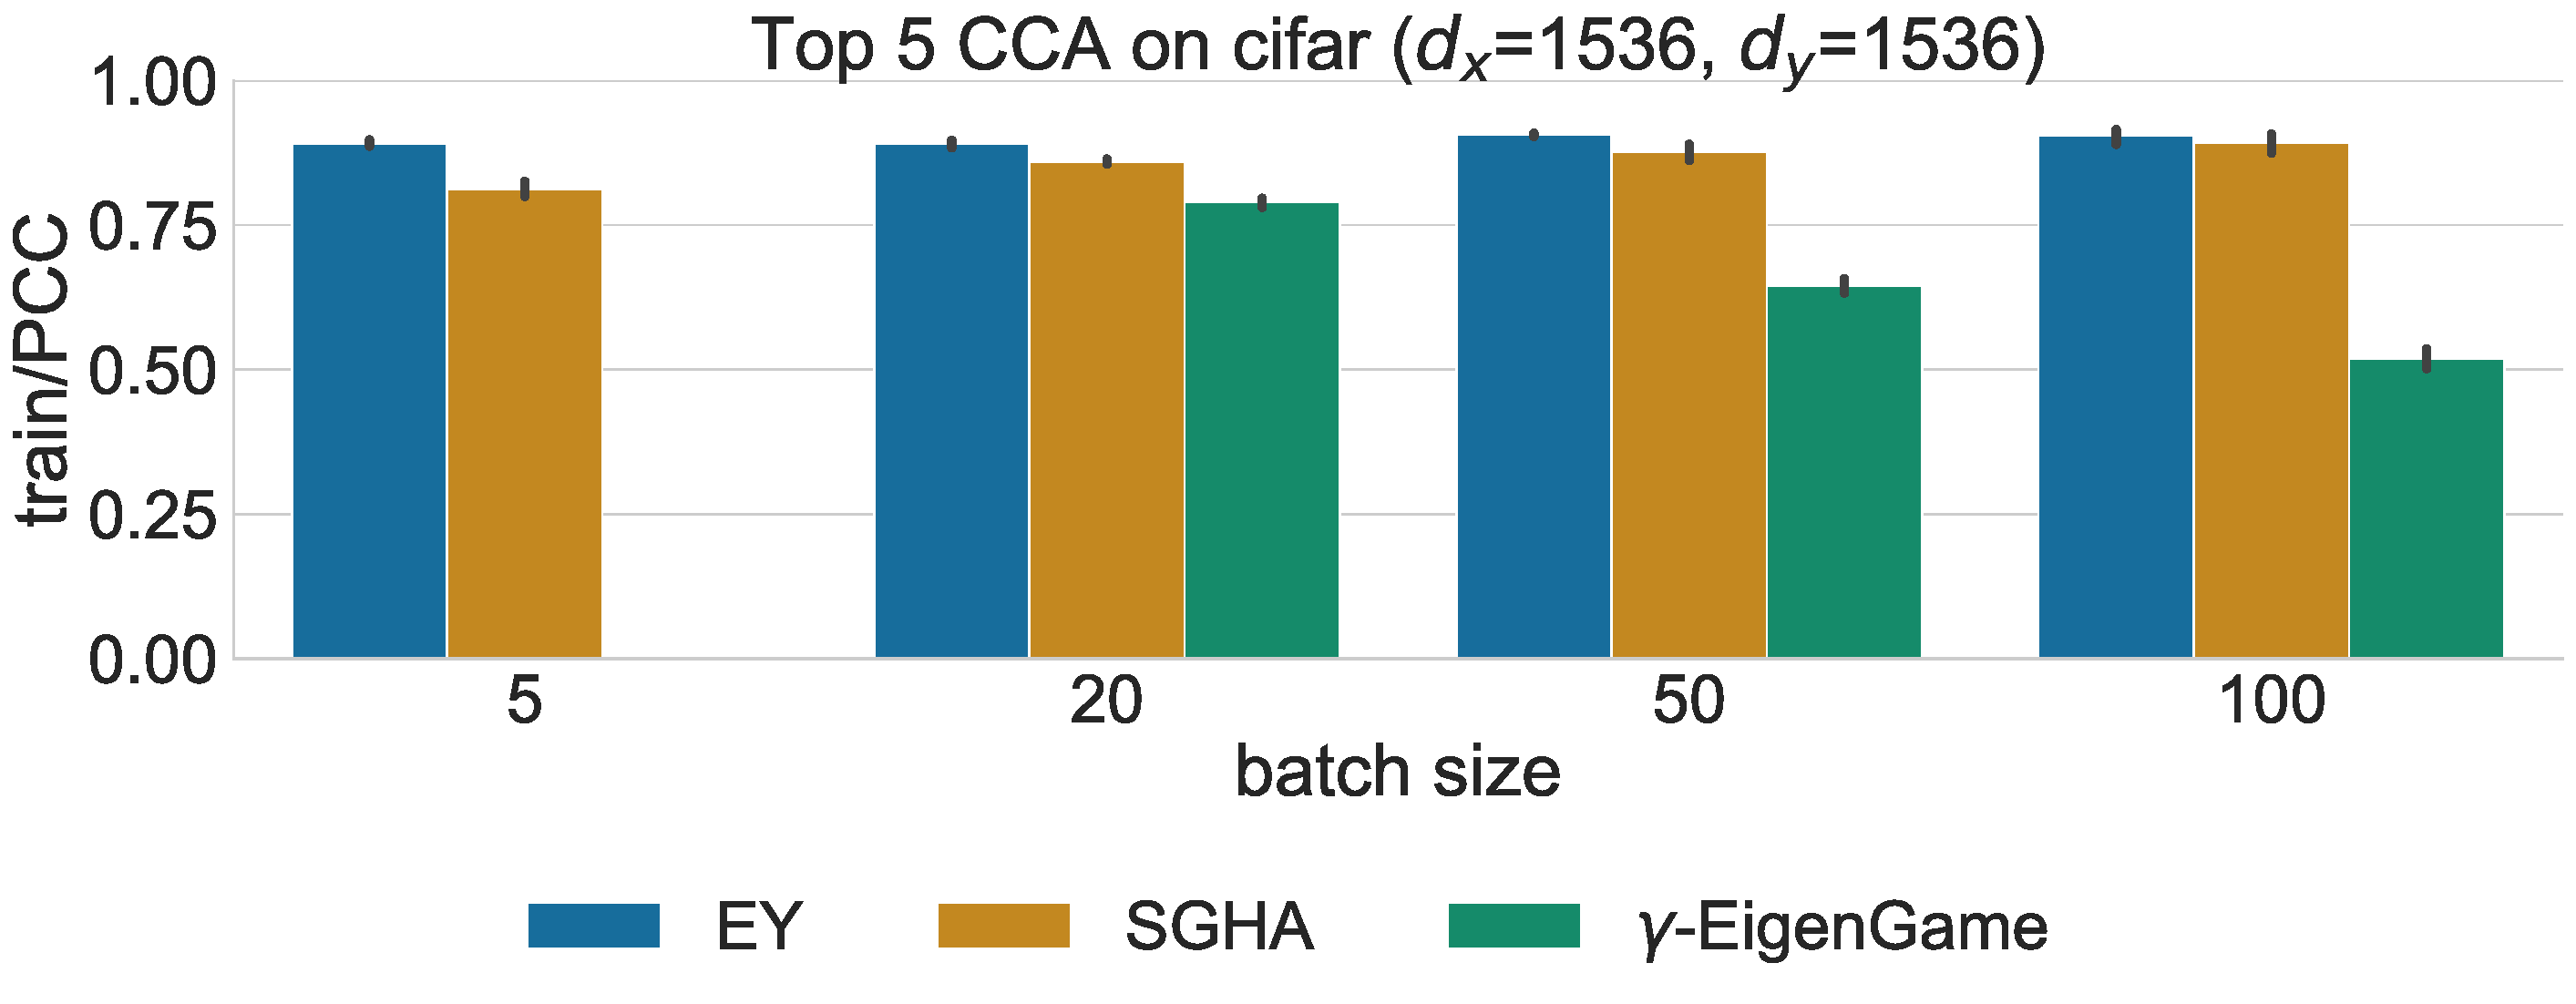
\includegraphics[width=0.6\textwidth]{figures/CCA/cifar_models_different_batch_sizes}
    \caption{Stochastic CCA on CIFAR using PCC: Performance across varying mini-batch sizes. Shaded regions signify \(\pm\) one standard deviation around the mean of 5 runs.}
    \label{fig:corr_cifar}
\end{figure}

\begin{figure}
    \centering
    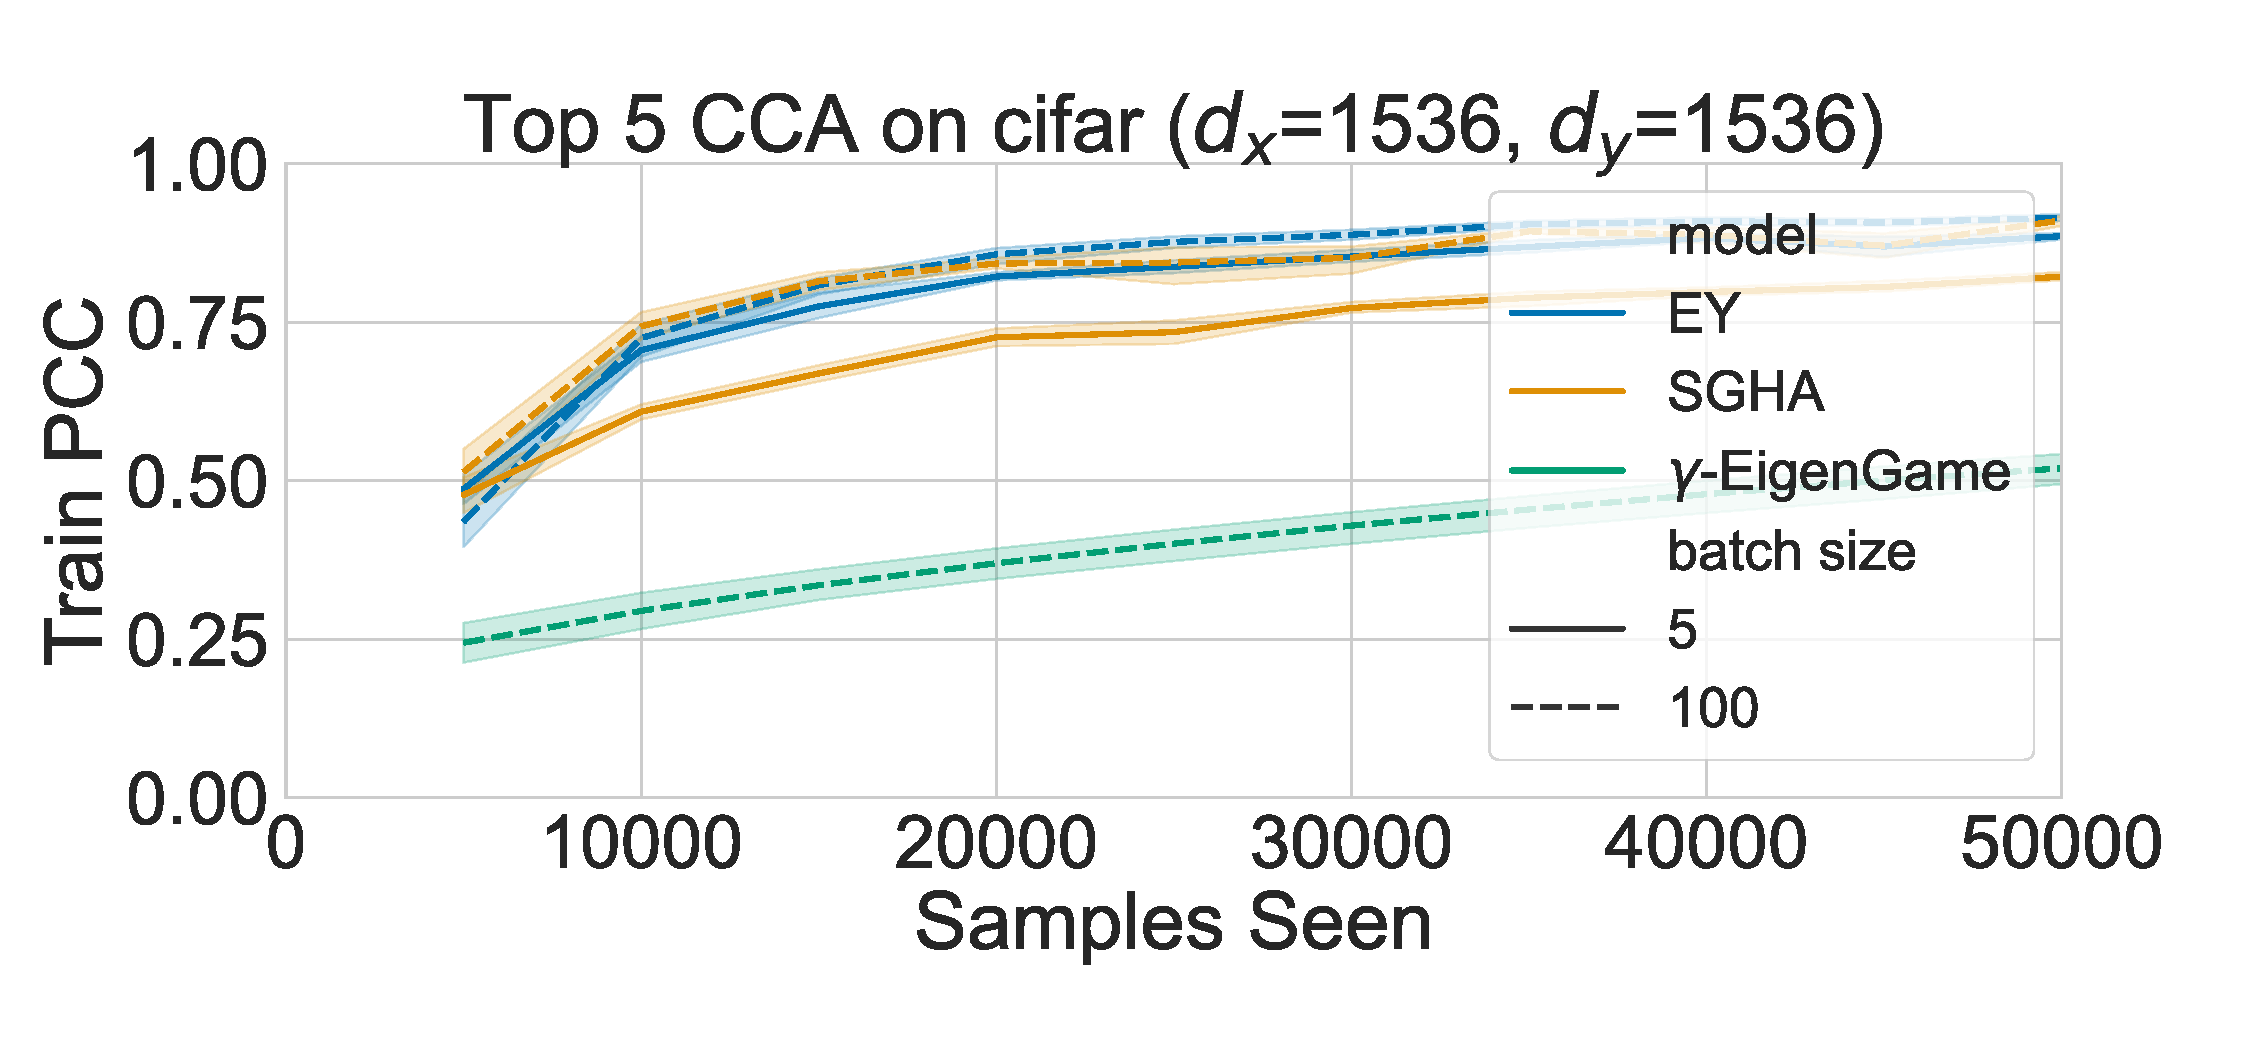
\includegraphics[width=0.6\textwidth]{figures/CCA/cifar_allbatchsizes_pcc}
    \caption{Stochastic CCA on CIFAR: Training progress over a single epoch for mini-batch sizes 5, 100.}
    \label{fig:learningcurve_cifar}
\end{figure}

\subsection{Stochastic PLS UK Biobank}
In this section, we aim to demonstrate the exceptional scalability and efficiency of our Stochastic PLS method, PLS-EY, in handling extremely high-dimensional imaging genetics data. We employ imaging genetics data from the UK Biobank \citep{sudlow2015uk} as our test bed, given its comprehensive and complex nature. The UK Biobank dataset presents a unique challenge due to the sheer scale of its genetic data, requiring sophisticated regularization strategies.

PLS is particularly suited for imaging-genetics studies due to its capability to handle high dimensionality and reveal novel phenotypes as well as genetic mechanisms underlying diseases and brain morphometry. Historically, imaging genetics analyses have been constrained to smaller datasets due to computational limitations \citep{Lorenzi2018,Taquet2021,Lefloch2012}. Moreover, the few studies that have attempted to analyze data of comparable scale to the UK Biobank have typically resorted to partitioning the data into smaller clusters, thereby limiting the scope of their analysis \citep{lorenzi2017secure, altmann2023tackling}.

Our experiment with PLS-EY, conducted on a subset of the UK Biobank dataset consisting of brain imaging data (82 regional volumes) and genetic data (582,565 variants) for 33,333 subjects, is designed to overcome these limitations. A particular computational challenge we address is maintaining orthogonality between the weight vectors \( u_k \) in the PLS model, which is crucial for the method's effectiveness. We run PLS-EY with a mini-batch size of 500 and train the GEP-EY PLS analysis for 100 epochs using a learning rate of 0.0001. This approach allows us to not only manage the high-dimensional nature of the data but also to preserve the integrity and interpretability of the analysis. To our knowledge, this represents the largest-scale PLS analysis of biomedical data to-date, showcasing the potential of our method to facilitate discoveries in extremely large datasets.

\paragraph{Data} The UK BioBank data consisted of real-valued continuous brain volumes and ordinal, integer genetic variants.
We used pre-processed (using FreeSurfer \citep{Fischl2012}) grey-matter volumes for 66 cortical (Desikan-Killiany atlas) and 16 subcortical brain regions and 582,565 autosomal genetic variants.
The affects of age, age squared, intracranial volume, sex, and the first 20 genetic principal components for population structure were removed from the brain features using linear regression to account for any confounding effects.
Each brain ROI was normalized by removing the mean and dividing the standard deviation.
We processed the genetics data using PLINK \citep{Purcell2007} keeping genetic variants with a minor allele frequency of at least 1\%  and a maximum missingness rate of 2\%.
We used mean imputation to fill in missing values and centered each variant.
To generate measures of genetic disease risk, we calculated polygenic risk scores using PRSice \citep{PRSice2014}.
We calculated scores, with a p-value threshold of 0.05, using GWAS summary statistics for the following diseases; Alzheimer's \citep{Lambert2013}, Schizophrenia \citep{Trubetskoy2022}, Bipolar \citep{Mullins2021}, ADHD \citep{Demontis2023}, ALS \citep{Van_Rheenen2021}, Parkinson's \citep{Nalls2019}, and Epilepsy \citep{International_League_Against_Epilepsy_Consortium_on_Complex_Epilepsies2018}, using the referenced GWAS studies.

\paragraph{Observations}
We observed strong validation correlations between all 10 corresponding pairs of representations \( Z^{(1)}_k \) and \( Z^{(2)}_k \) in the PLS model, with weak cross-correlations between \( Z^{(1)}_k \) and \( Z^{(2)}_i \) for \( i \neq k \). This indicates that our model learned a coherent and orthogonal subspace, as shown in Figure \ref{fig:UKBB_corr}. Furthermore, the PLS representations \( Z \) were significantly associated with genetic risk measures for several disorders, suggesting that the learned PLS subspace encodes relevant information for genetic disease risk, a critical insight for biomedical research (Figure \ref{fig:genetic_risk}). These results demonstrate the scalability of our method to extremely high-dimensional data, and its ability to learn interpretable representations.

\begin{figure}
    \centering
    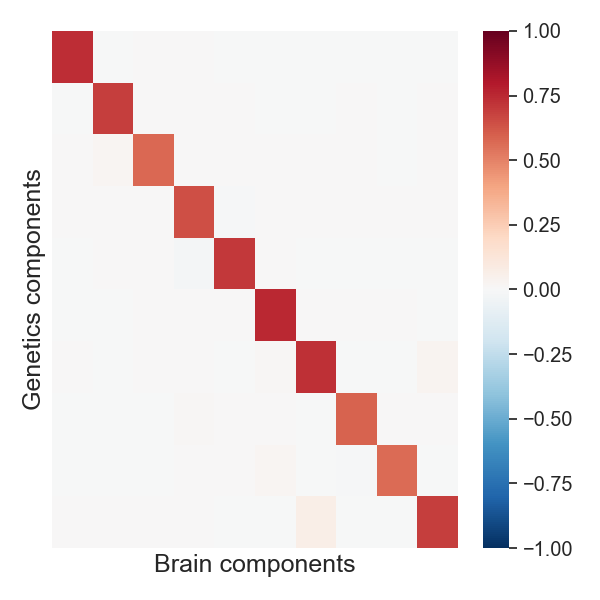
\includegraphics[width=0.6\textwidth,trim={0.8cm 0cm 0.3cm 0cm}]{figures/UKBB/cross_corr.png}
    \caption{Pearson correlations among PLS latent variables \( Z_k \) derived from UK Biobank data.}
    \label{fig:UKBB_corr}
\end{figure}

\begin{figure}
    \centering
    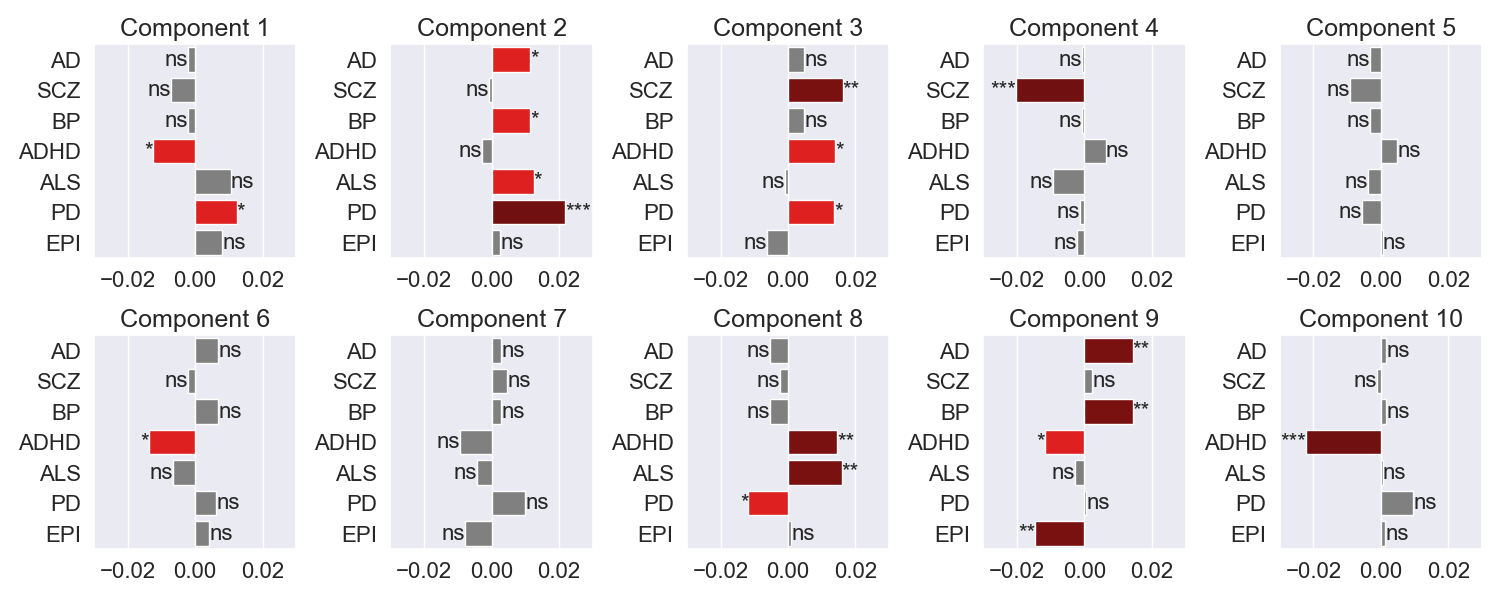
\includegraphics[width=0.6\textwidth,trim={0.5cm 0cm 0.7cm 0cm}]{figures/UKBB/prs_correlations.png}
    \caption{Correlation between PLS brain representations \( Z \) and genetic risk scores for various disorders. AD=Alzheimer's disease, SCZ=Schizophrenia, BP=Bipolar, ADHD=Attention deficit hyperactivity disorder, ALS=Amyotrophic lateral sclerosis, PD=Parkinson's disease, EPI=Epilepsy. $\text{ns}: 0.05< p \leq 1, \ast: 0.01< p \leq 0.05, \ast\ast: 0.001< p \leq 0.01, \ast\ast\ast: 0.0001< p \leq 0.001$.}
    \label{fig:genetic_risk}
\end{figure}


\section{Conclusion}

In this chapter, we introduced a class of efficient, scalable algorithms for Canonical Correlation Analysis, and Generalized Eigenvalue Problems more broadly, rooted in a novel unconstrained loss function.
These algorithms are computationally lightweight, making them uniquely suited for large-scale problems where traditional methods struggle.